\subsection{Introduction to the Choicely voting platform}
    % what does the company do? 
    Choicely \footnote{\url{http://choicely.com/}} is a voting platform developed by the Finnish Lovented Ltd since 2014. The software provides the possibility for users to engage in interesting contests by voting on their favorite contender. The platform has already hosted numerous contests in various fields, such as beauty pageants, public polls, design contests, talent shows, sport events among many others. The customer base of the firm consist of mainly Finnish broadcasters, publishers and advertisers. However, the recent years have brought numerous users and customers from all around the world.
    
    % what are the contests like, what kind of configuration settings are available?
    % The contests in the platform are created by users or brands. 
    Contests hosted in Choicely can be divided into generally two groups:
    
    \begin{enumerate}
        \item voting contests: the contest organizer provides the participants to the contest. This way the list of participants cannot be changed as soon as a contest is created.
        \item challenge contests: the public provides the participants to the contest. The list of participants may change over time depending on how many users would like to join with their own content. 
    \end{enumerate}
    
    % voting options
    Various voting options are available for both contest types. The author of the contest has the choice of setting a limit on how many votes users can spend on individual participants or the whole contest in overall. For instance, if the maximum votes in the contest is set to 1, users can give exactly one vote on one and only one participant. Configuration settings allow infinite votes as well. For instance, users may vote on all of the participants as many times as they like in a talent show in this case. Removing votes is possible, if the author has decided to enable this possibility. Votes cannot be modified after the contest has ended. Each contest has its own voting configuration.
    
    % free-silver-gold votes
    On top of the regular free votes, contest authors may allow users to earn more votes (called "silver votes") by sharing the contest on social media or by watching advertisements. Furthermore, contest authors can allow users to purchase more votes (called "star votes" or "gold votes") with exactly the same restriction settings as explained above. Note, however that the configuration for the three vote types are distinct for every contest. This means that the limitation on free/silver/star votes may differ for individual participants as well as the whole contest. For instance, a contest author may allow users to spend only 5 votes for free, but unlimited number of silver and gold votes in a contest.

    % how can one reach a contest in the platform?
    Contests can be accessed through multiple interfaces (Figure \ref{choicely_platforms}). Naturally, the company's webpage provides a convenient way to create, browse and participate in contests. Choicely also has free mobile applications available on Android and iOS devices, that can be installed through the Google Play \footnote{\url{https://play.google.com/store/apps/details?id=com.choicely.android}} and the iOS App Store \footnote{\url{https://itunes.apple.com/fi/app/choicely/id1158798364}} on the devices. Finally, the company offers a web widget, which can be embedded as a framework in any webpage easily. The last option is often used by many of Choicely's customers, because it provides a convenient way to embed rich content in their own web pages, which users are already familiar with. Users may vote and participate in their own contests if they like. Users may participate in arbitrary number of contests from three platforms: the two most popular mobile platforms (iOS and Android) and the web interface. 
    
    \begin{figure}[h] 
        \begin{center}
            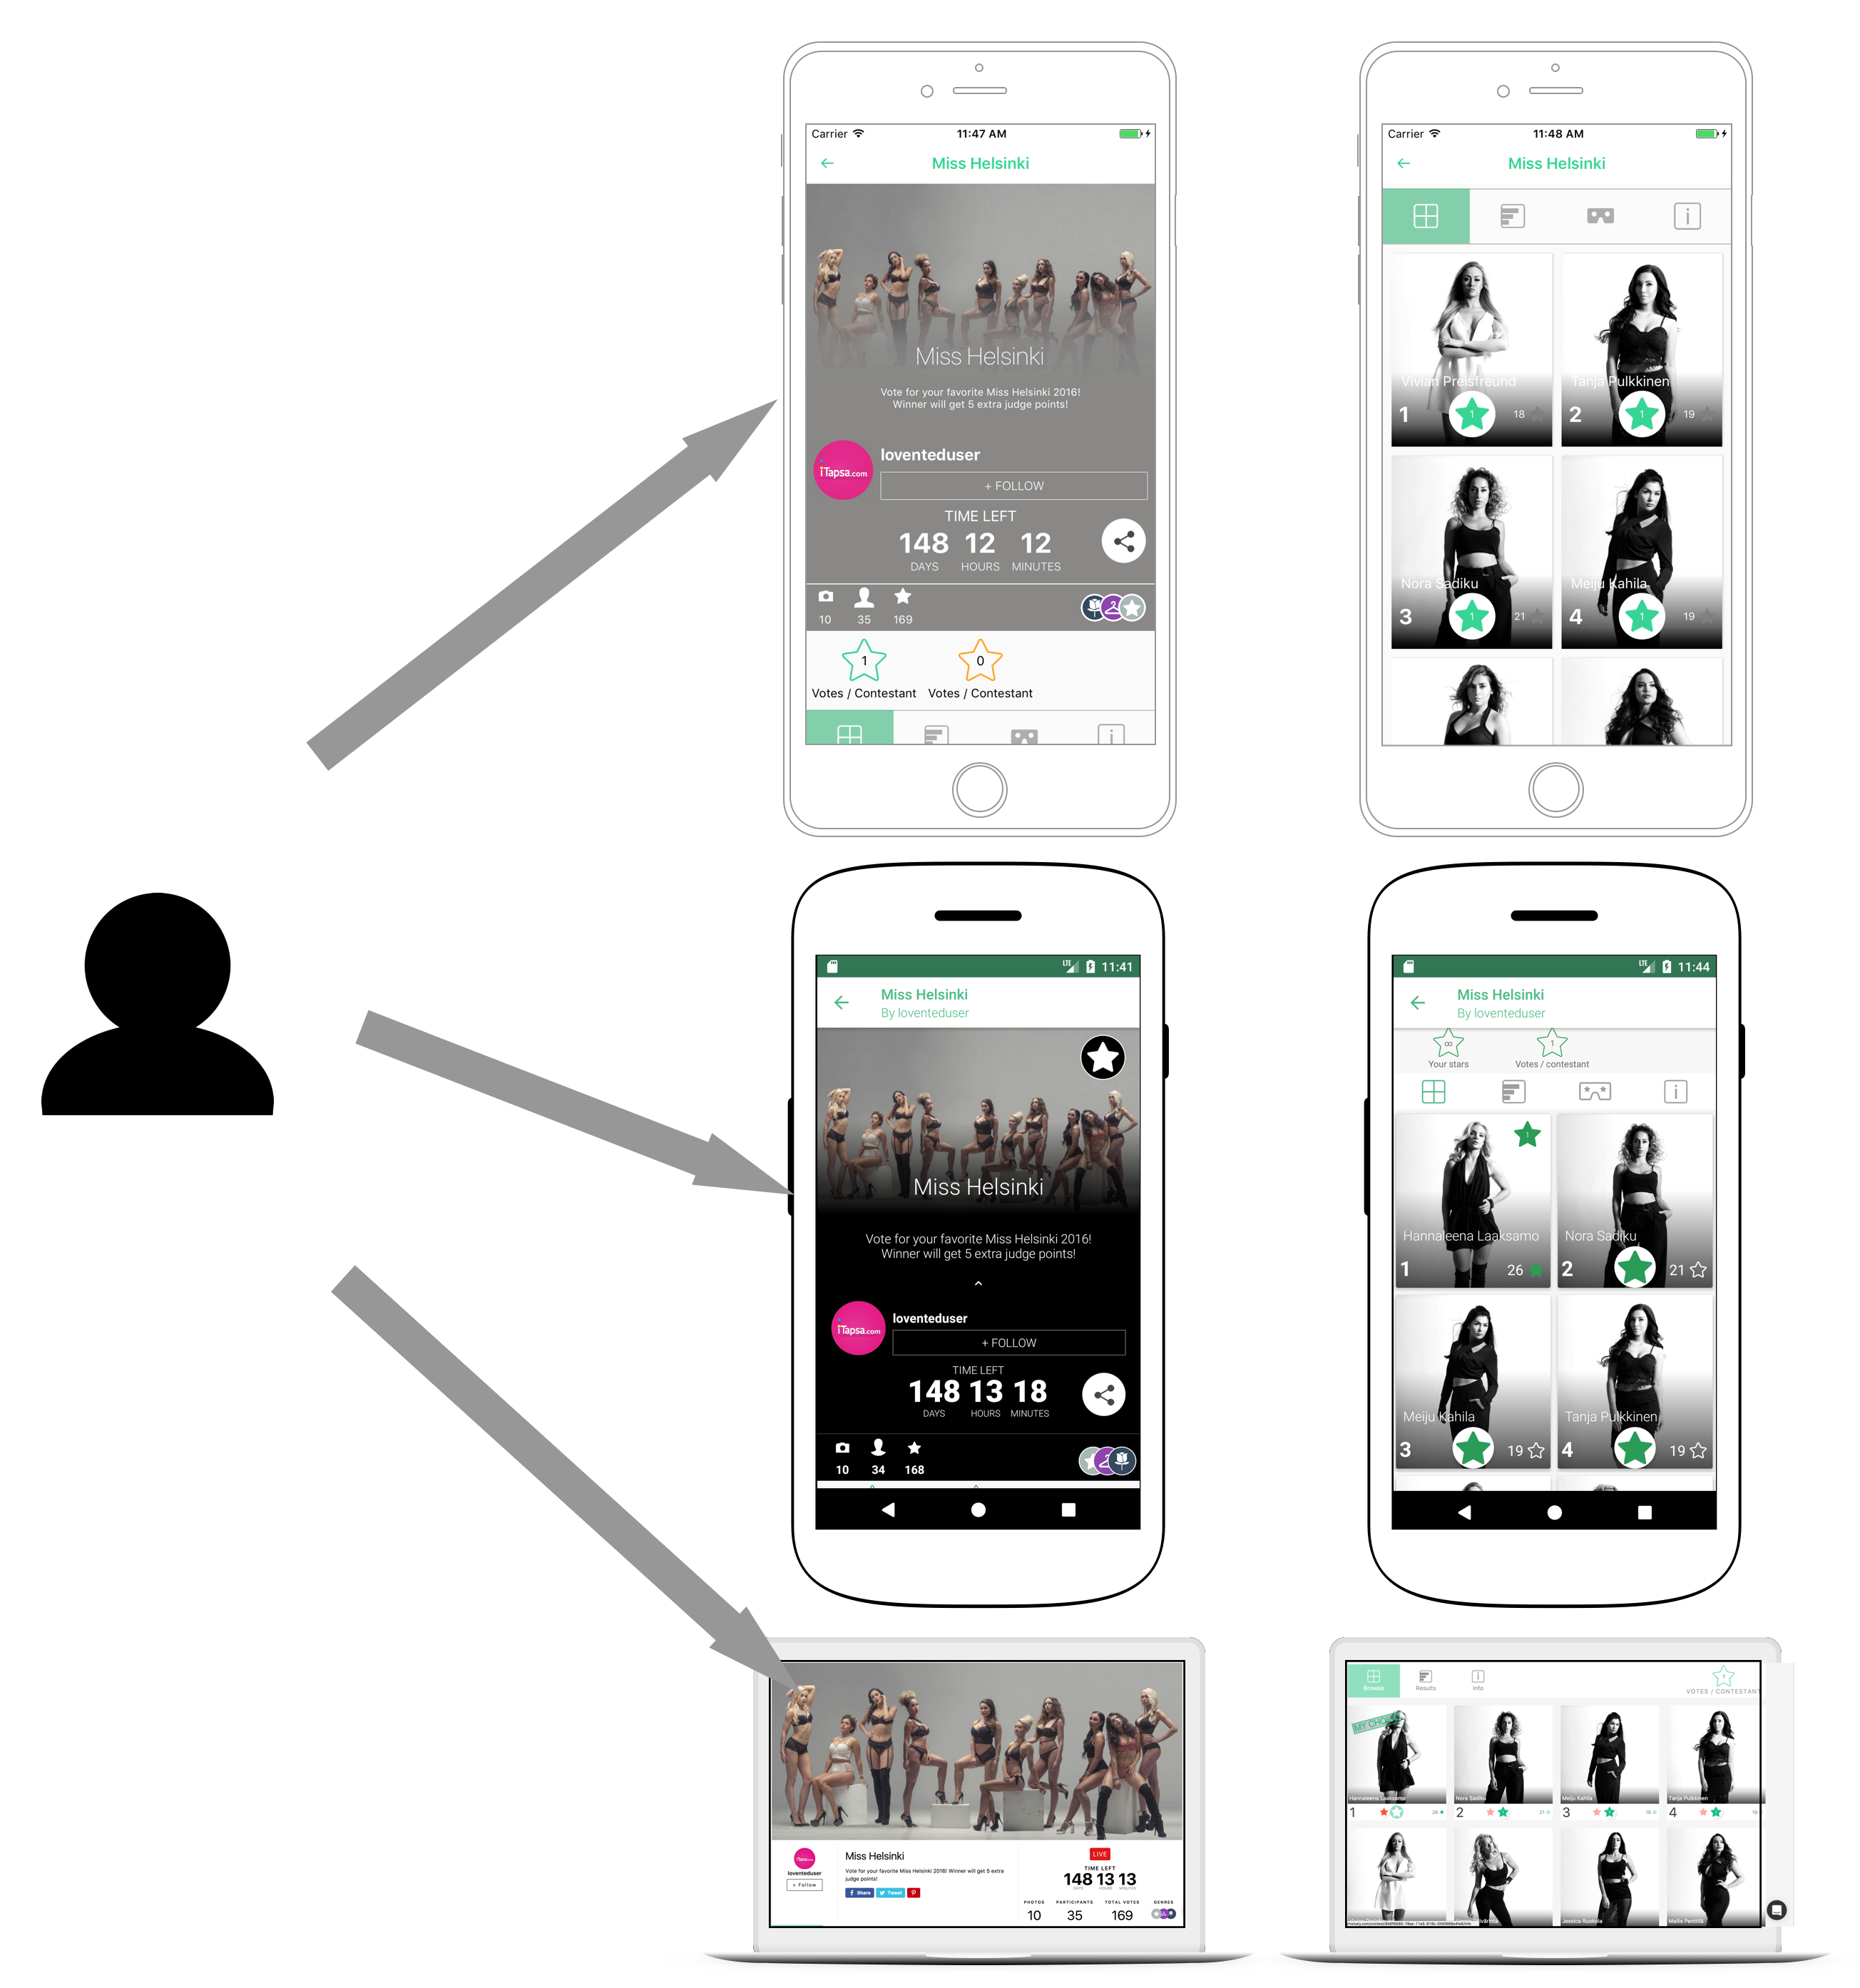
\includegraphics[width=0.6\textwidth]{images/choicely_platforms.png}
            \caption{Users can vote in contests through three interfaces: iOS devices, Android devices and web.}
            \label{choicely_platforms}
        \end{center}
    \end{figure}

    % what do users have to do to participate? 
    Majority of the contests require users to have a user profile in the Choicely platform. Choicely offers authentication through social media (Facebook and Google+) as a convenient option for users to sign up with one click. Optionally, user profiles can be created through a regular sign-up process, where users pick a username as their identities. When users choose this kind of registration, their e-mail addresses are confirmed through a verification link sent to their inbox, so that their identity is confirmed. Each user profile contains the features listed in Table \ref{user_profile_fields}. 

    \begin{table}[]
        \centering
        \begin{tabular}{l|l}
            \textbf{Field}              & \textbf{Type} \\
            \hline
            Full name                   & Free text \\
            Profile picture             & Image \\ 
            Cover image                 & Image \\
            Gender                      & Male/Female/Other/Not specified \\
            Location                    & Country, state and city \\
            Birthday                    & Datetime \\ 
            Age group                   & 0-17/18-24/25-34/35-44/45-54/55-64/65+ \\
            Introduction/Bio            & Free text
        \end{tabular}
        \caption{The list of fields and their types for each user profile.}
        \label{user_profile_fields}
    \end{table}

    % other contest-related data
    Contests also have some meta data which can facilitate data analysis. Each contest belongs to at least one but up to three of the following categories: animals, beauty, danger, design, entertainment, fashion, food, games, humor, sports, travel, other. The category labels are aligned by the contest's author upon creation. Contests also have starting and an ending time, between which users can vote or participate in them. While votes arrive into a contest, the vote count value tells the number of total votes received, while the number of unique voters tells how many individual users have voted in the contest.   

    % what kind of data is generated?
    Consequently, the available data is two-folded: the user profiles contain demographic information about the users (age group, gender and location), while contests have a number of participants with arbitrary number of votes that the users have spent on them. The latter kind of data can be seen as digital footprints generated by users in the Choicely platform. The combination of these datasets sums up to the user data as explained in the previous chapter and Figure \ref{user_data_venn} in this particular case. This is further supported with the meta data of contests explained in the previous paragraph. 

    %The vote changes for the contests are stored as transactions. This means that the database contains not the final results of the voting, but rather the changes what users made while using the software. This way it is possible to analyze the votes over time and to look at changes individually. For instance, it is possible to tell if a user has removed his/her votes from participant A and moved them to participant B. Furthermore, this way of data representation to restore or simulate any previous state of the contest, in case it would be needed.

\subsection{Research setting}
    % why is the data analysis relevant from scientific research point of view?
    Performing scientific research on such data is interesting for multiple reasons. To begin with, at the time of this research Choicely does not utilize data analysis tools to gain better understanding on the collected data. It is in the interest of the company and its customers to better understand what kind of audience was engaged in the past, what kind of content is more (or less) successful and what tendencies in user behavior can be extracted from the data. As a result, the introduction of data analysis and visualization tools at the company will greatly enhance business value of the firm, provide deeper understanding on the domain as well as the existing user base.   
    
    % how is Choicely different than other social networks or any other repository of user data?
    Secondly, Choicely can be looked at as a social network, because some of the platform uploaded to the platform is generated by users. Users also have the possibility to express their appreciation or support towards some contest participants by spending votes on them. Similarly to social networking sites, where the "like" feature is often used \cite{jang2015noreciprocity, bakhshi2014faces} this phenomena can be looked at as a way of expressing personal opinion. 
    
    In comparison to most of the currently available social networks, voting platforms like Choicely are observed by the audience differently. On one hand, social media sites usually list posts or images on a feed, where there is theoretically no relation between the posts that follow eachother. On the other hand, contestants in the Choicely platform share similarities as they were nominated for the same contest. Accordingly, there must be some similarity among them as all are subjects of the contest's topic, rules and are competing for the best possible result. 

    % so what? Why is that important from user point of view
    This slight difference in the content makes a big change in terms of user behavior. The focus moves from "what kind of content I like" to "which piece of content I like the most in comparison to the rest". Consequently, users will scan through some (or optimally all) of the contestants and make unconscious decisions upon whether to give vote(s) on certain contest participant(s). The users express their favour and support towards a subset of contenders, and hence helping them to reach their ultimate goal: winning in the contest. 
    % how can this contribute to user behavior and social media studies? 
    This difference compared to other social networking sites offers a great possibility for research. The potential of identifying what kind of content among different contests individuals like as well as what kind of content similar group of users like, hinders in the data.    

    % how computer vision is going to be utilized? 
    One of the challenges in connecting users with topics of contests is that there is no indication on what the content on the contenders' pictures is. Contest authors only assign categories to the contests to be created, which does not necessarily describe the entrants in the contest. Other researches have successfully utilized computer vision to gather meta data for the uploaded content in image sharing communities \cite{bakhshi2014faces, hu2014we}. 
    
    % what is the solution to this problem?
    Deriving from the success in previous studies \cite{hu2014we, farseev2015harvestingmultiplesources, han2016teensarefrommars, bakhshi2014faces}, computer vision is utilized in this research to identify labels that appear on the participants' images. For instance, a beauty pageant's entry image may be labelled with meta data, such as "Beauty", "Photo Shoot", "Smile" and "Blonde". Similarly, a design contests entry might have topic labels, such as "Landmark" or "Architecture". Figure \ref{google_vision_labels} displays an example, where the Google Vision API was used to extract such labels from images, that were participants in two of Choicely's contests.

    \begin{figure}[h] 
		\begin{center}
            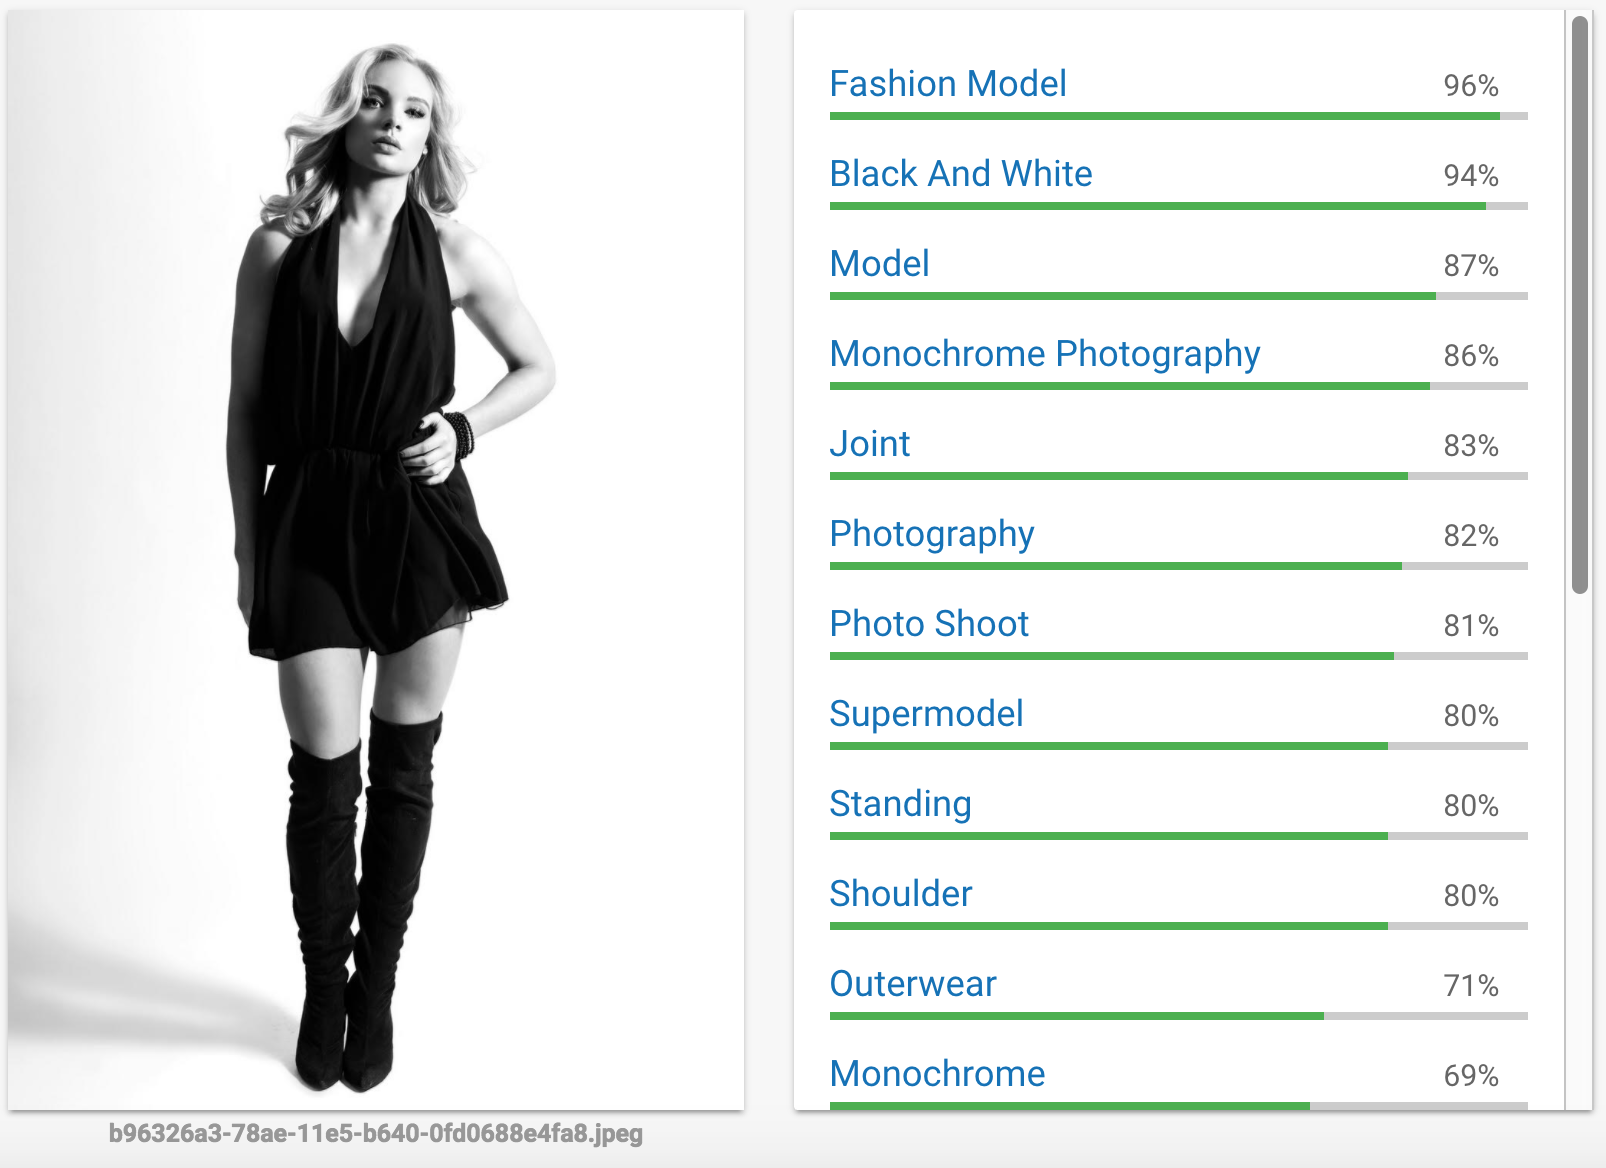
\includegraphics[width=0.8\textwidth]{images/google_vision_labels.png}
            
\includegraphics[width=0.8\textwidth]{images/google_vision_labels2.png}
			\caption{The labels identified by the Google Vision API on two of the contest participant's images.}
			\label{google_vision_labels}
		\end{center}
    \end{figure}

    % how are the labels used - what is the method performed on them? 
    Combining the identified labels and the vote data can provide information on user behavior. For instance it can be identified which demographic group of users like what kind of content, or the behavioral differences between two or more groups can be compared to eachother. Furthermore, this kind of information could be used to recommend new content in the platform to users which they have not seen before. Last but not least, it could be identified that which traits of participants contribute to more votes and engagement by users or certain user groups.  
    
    \subsection{Data structure}
    % architectural overview
    The current architecture of the Choicely platform is...
    \begin{figure}[h] 
		\begin{center}
            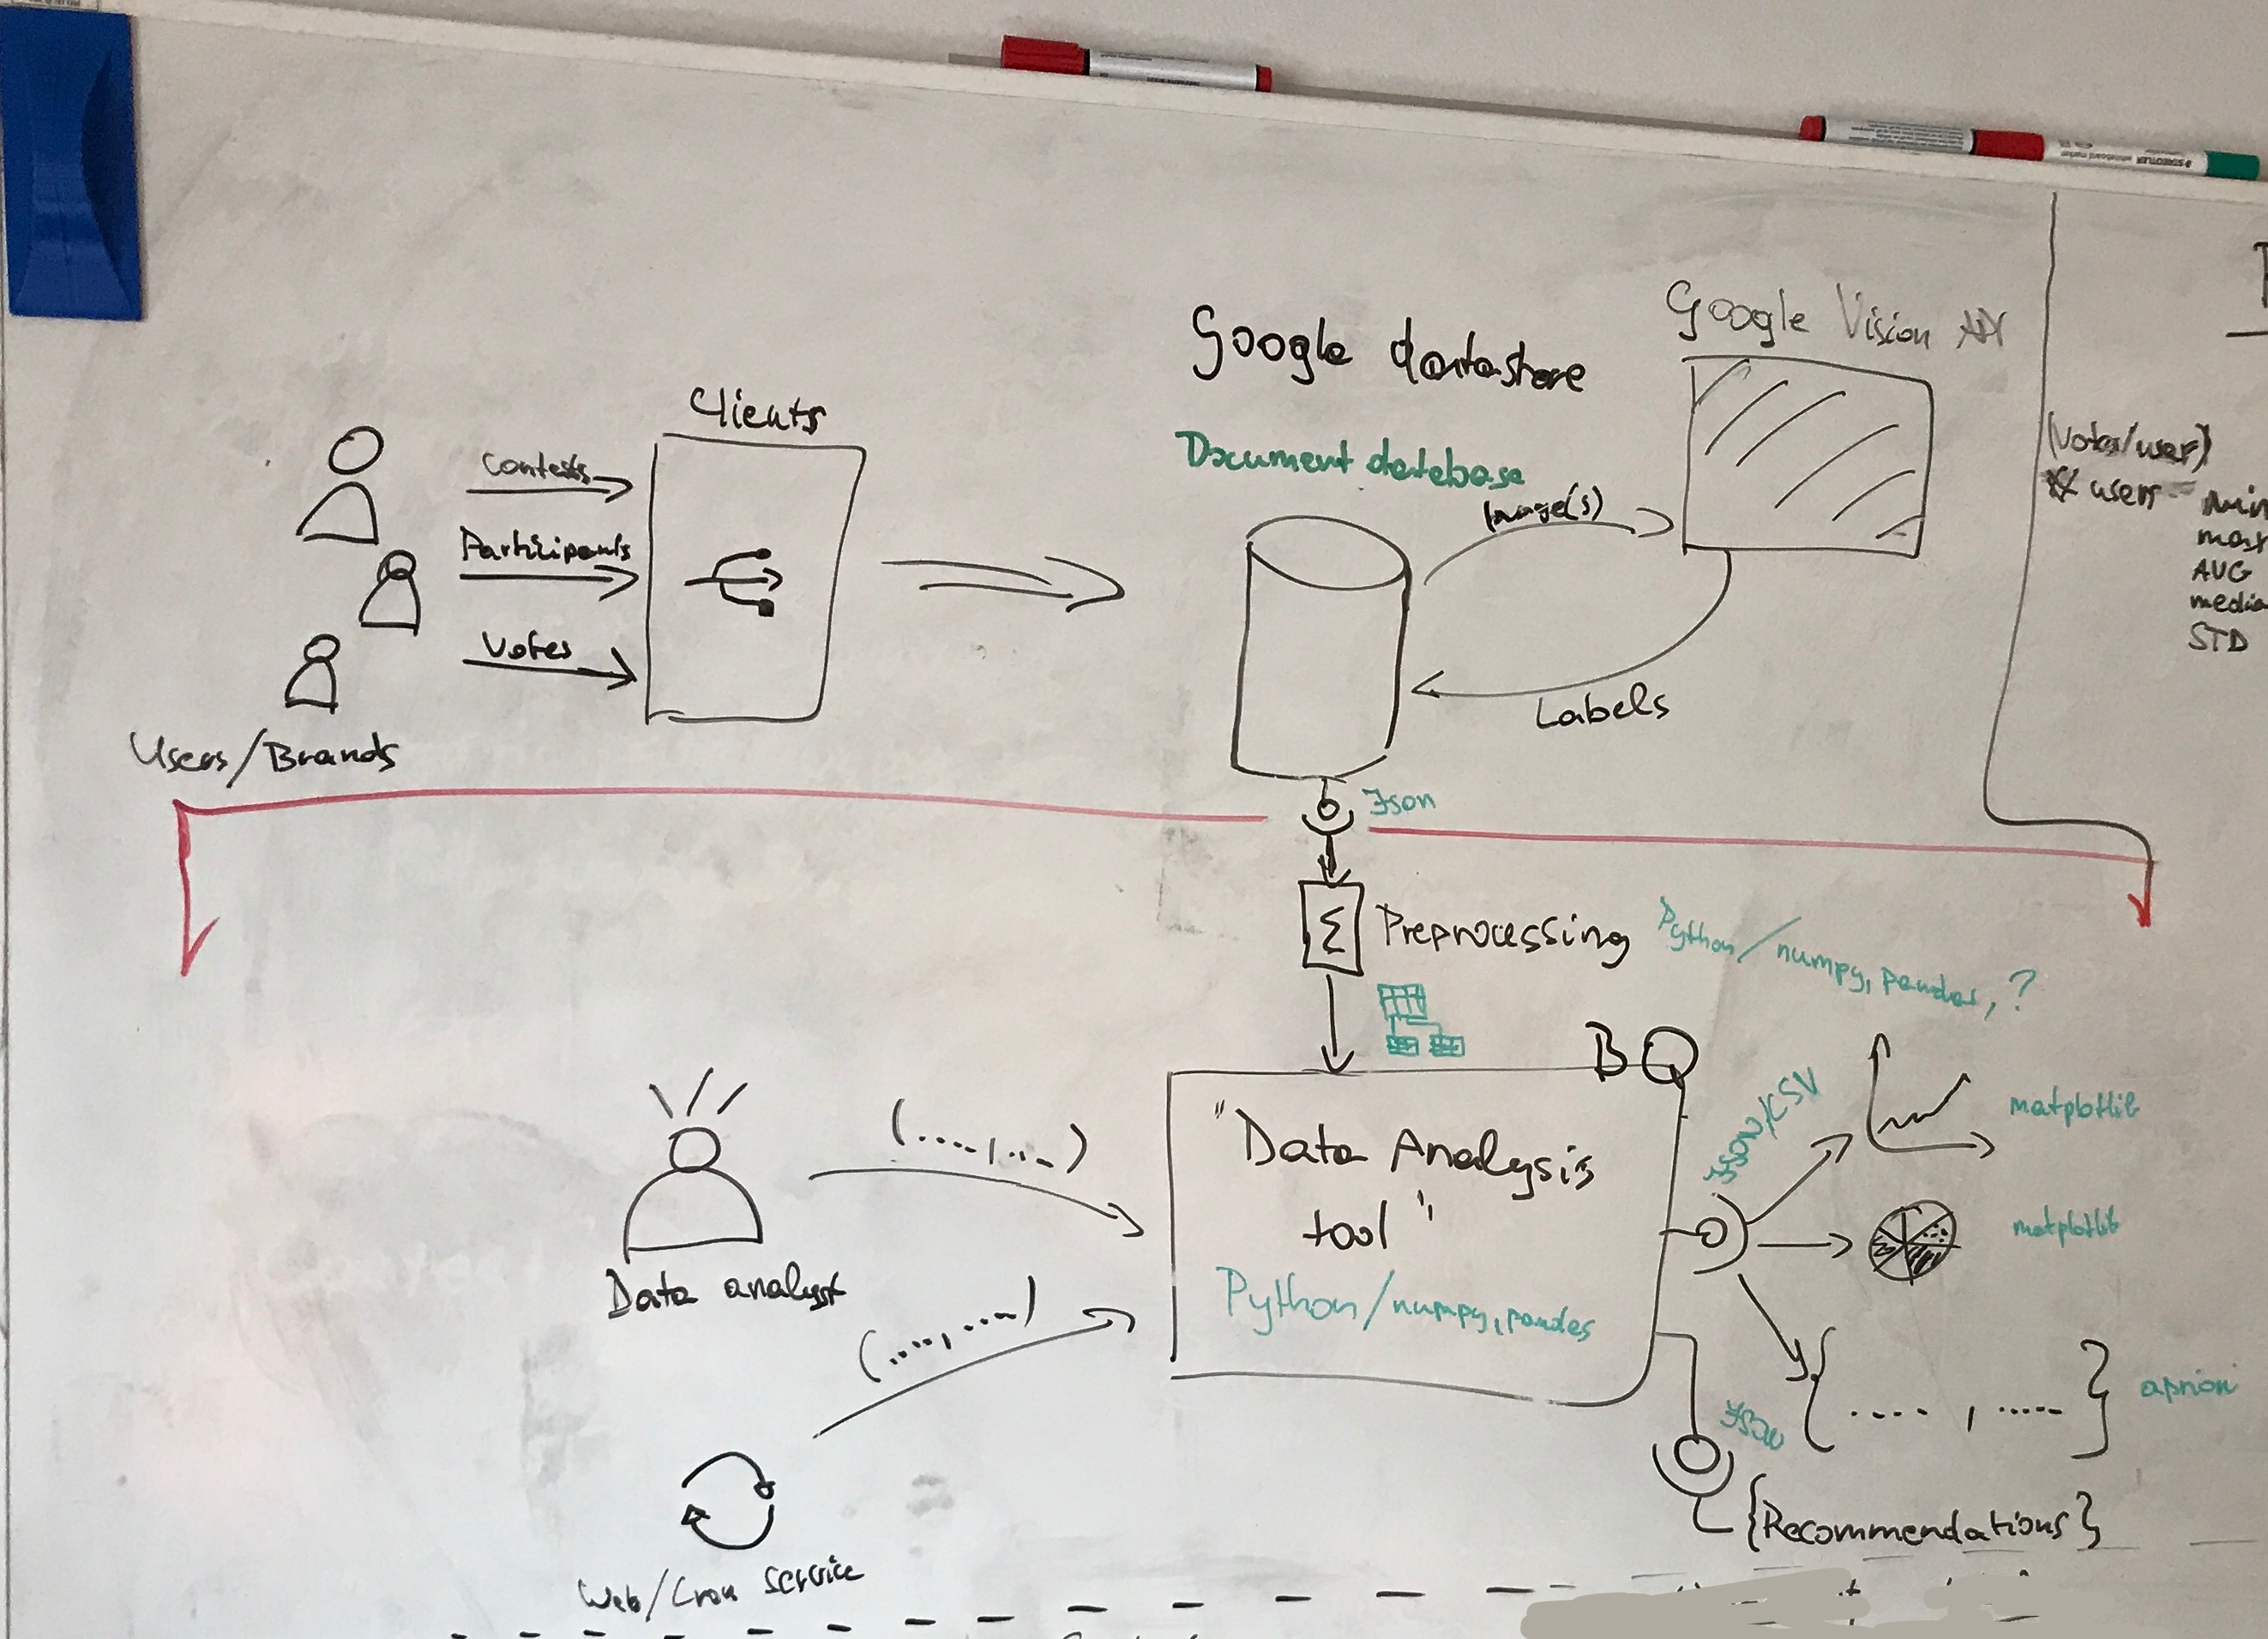
\includegraphics[width=0.8\textwidth]{Images/architecture_whiteboard.jpg}
			\caption{The brief architectural overview of the Choicely platform.}
			\label{choicely_architecture}
		\end{center}
    \end{figure}

    \begin{figure}[h] 
		\begin{center}
            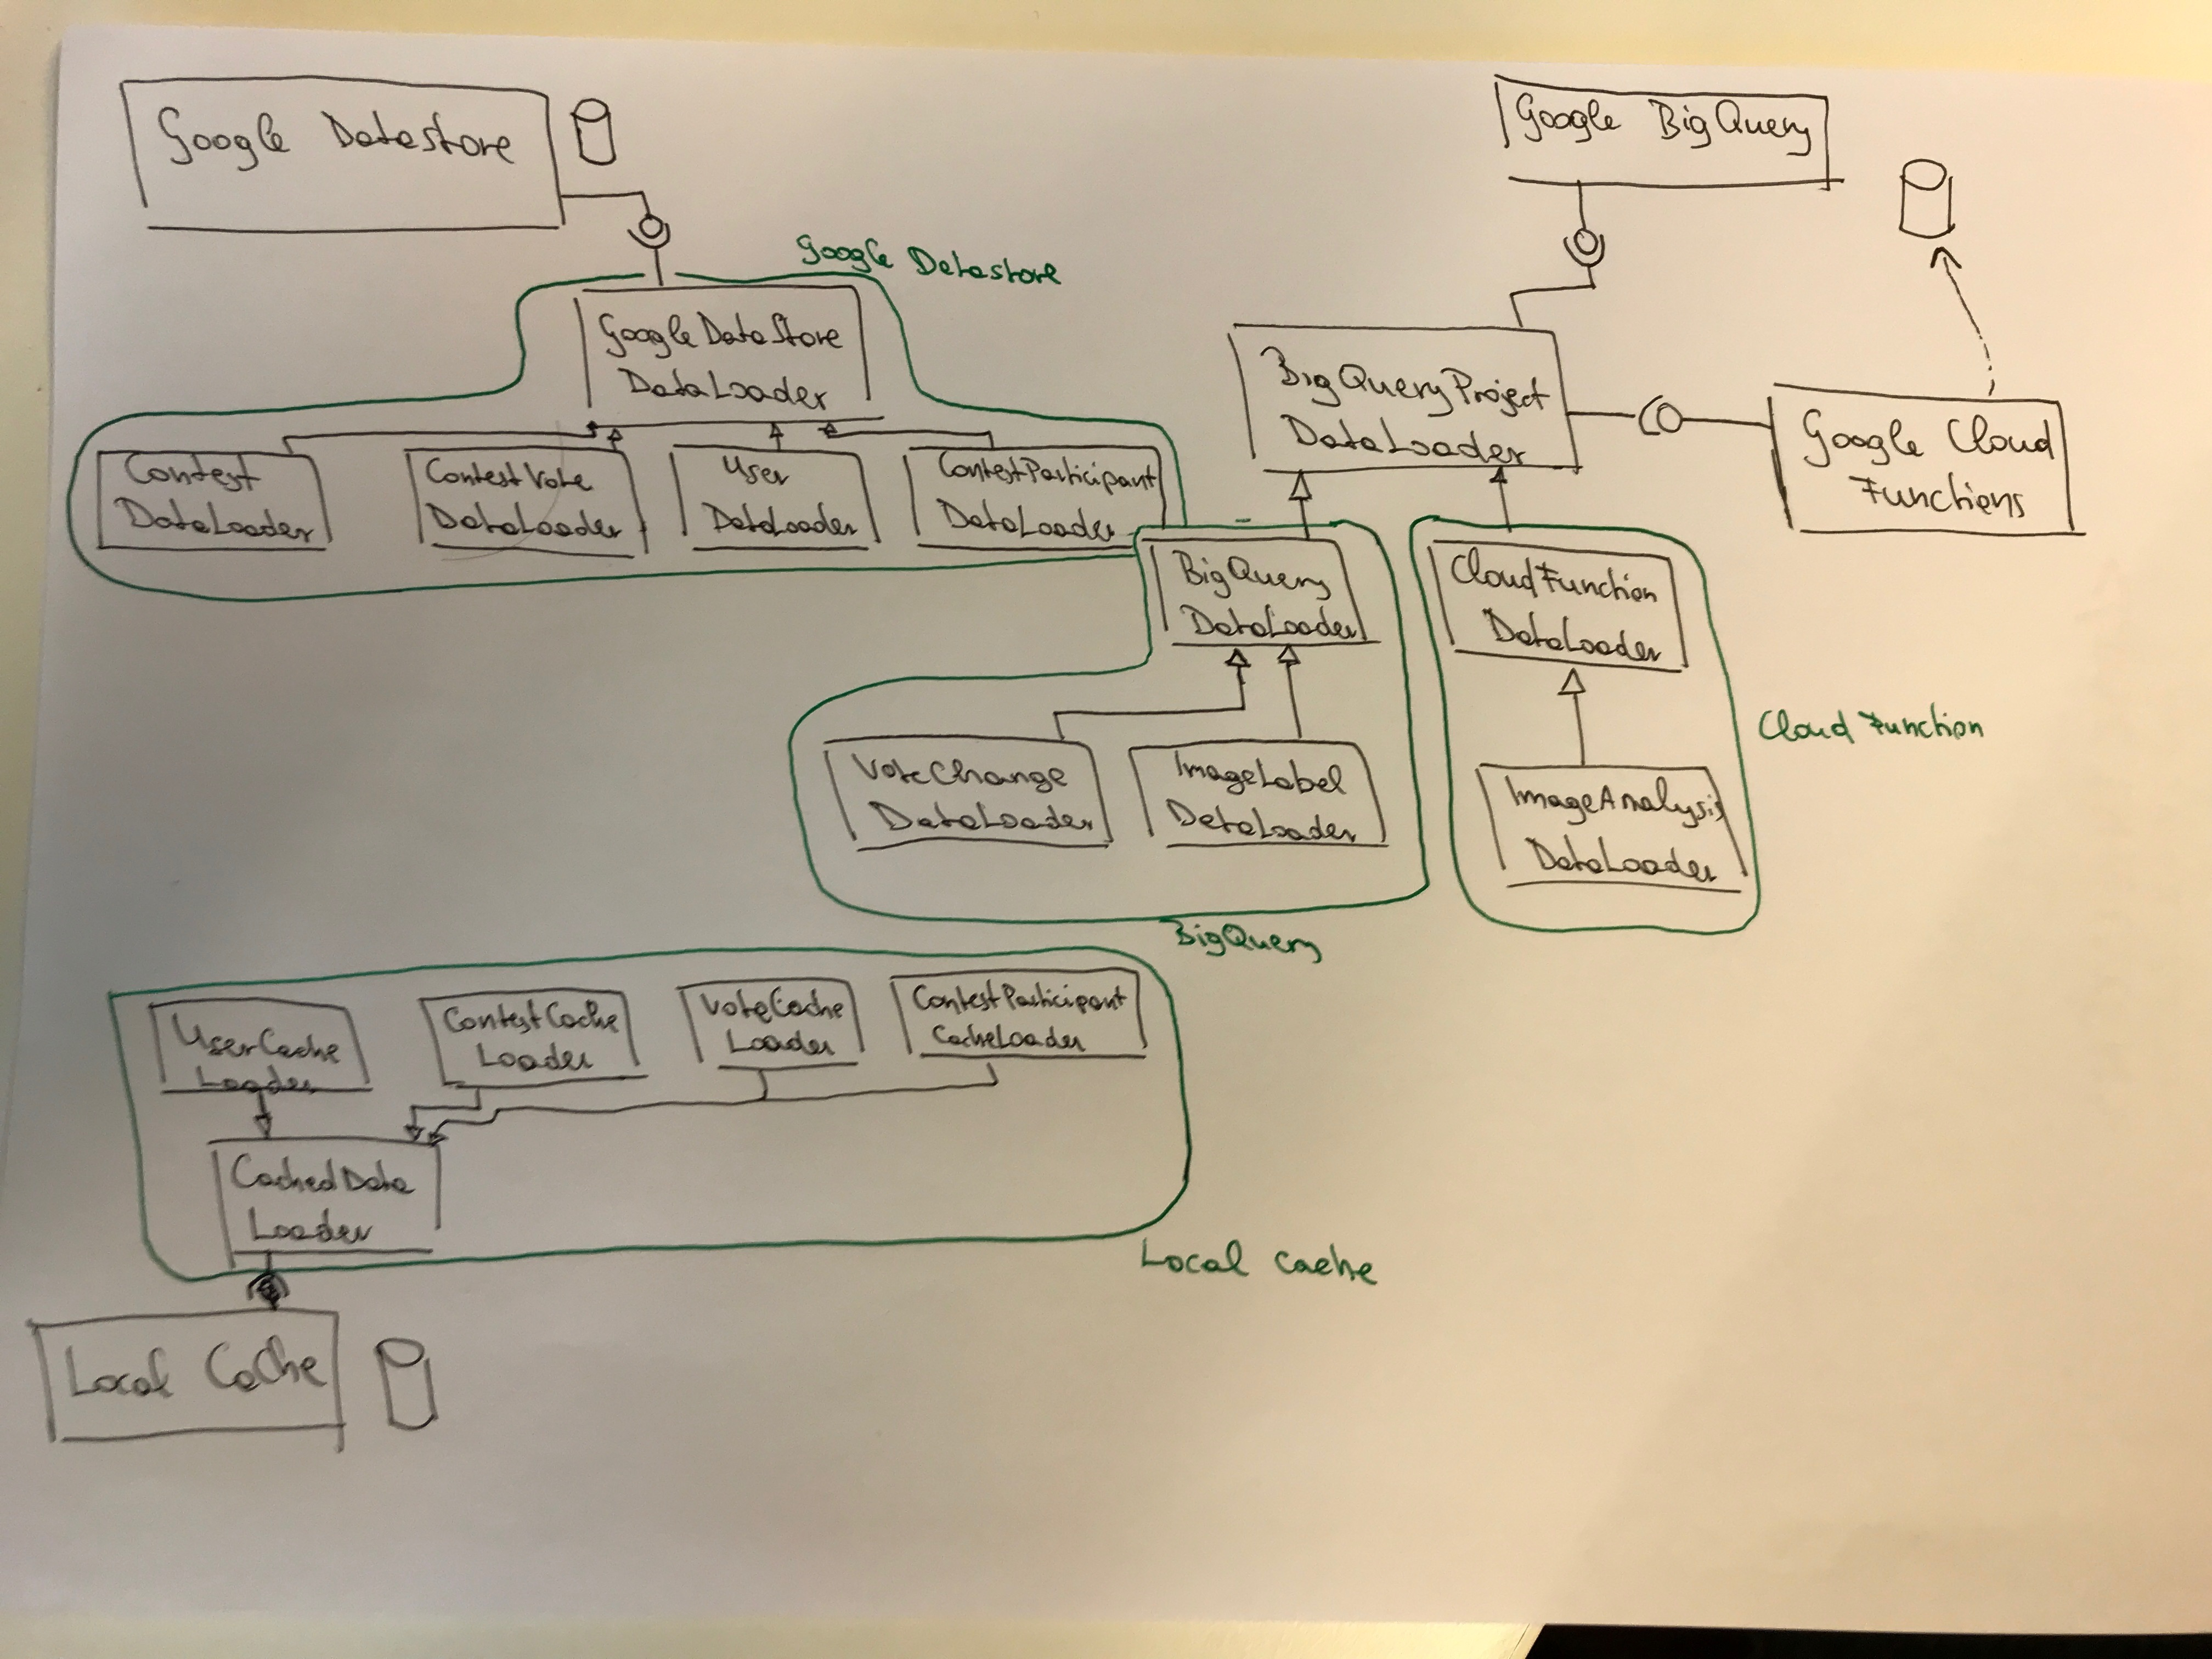
\includegraphics[width=0.8\textwidth]{Images/IMG_1317.jpg}
			\caption{The data sources of the data analysis in the Choicely platform.}
			\label{choicely_data_sources}
		\end{center}
    \end{figure}

    % the structure of the data models
    The structure of the data... 
    \begin{figure}[h] 
		\begin{center}
            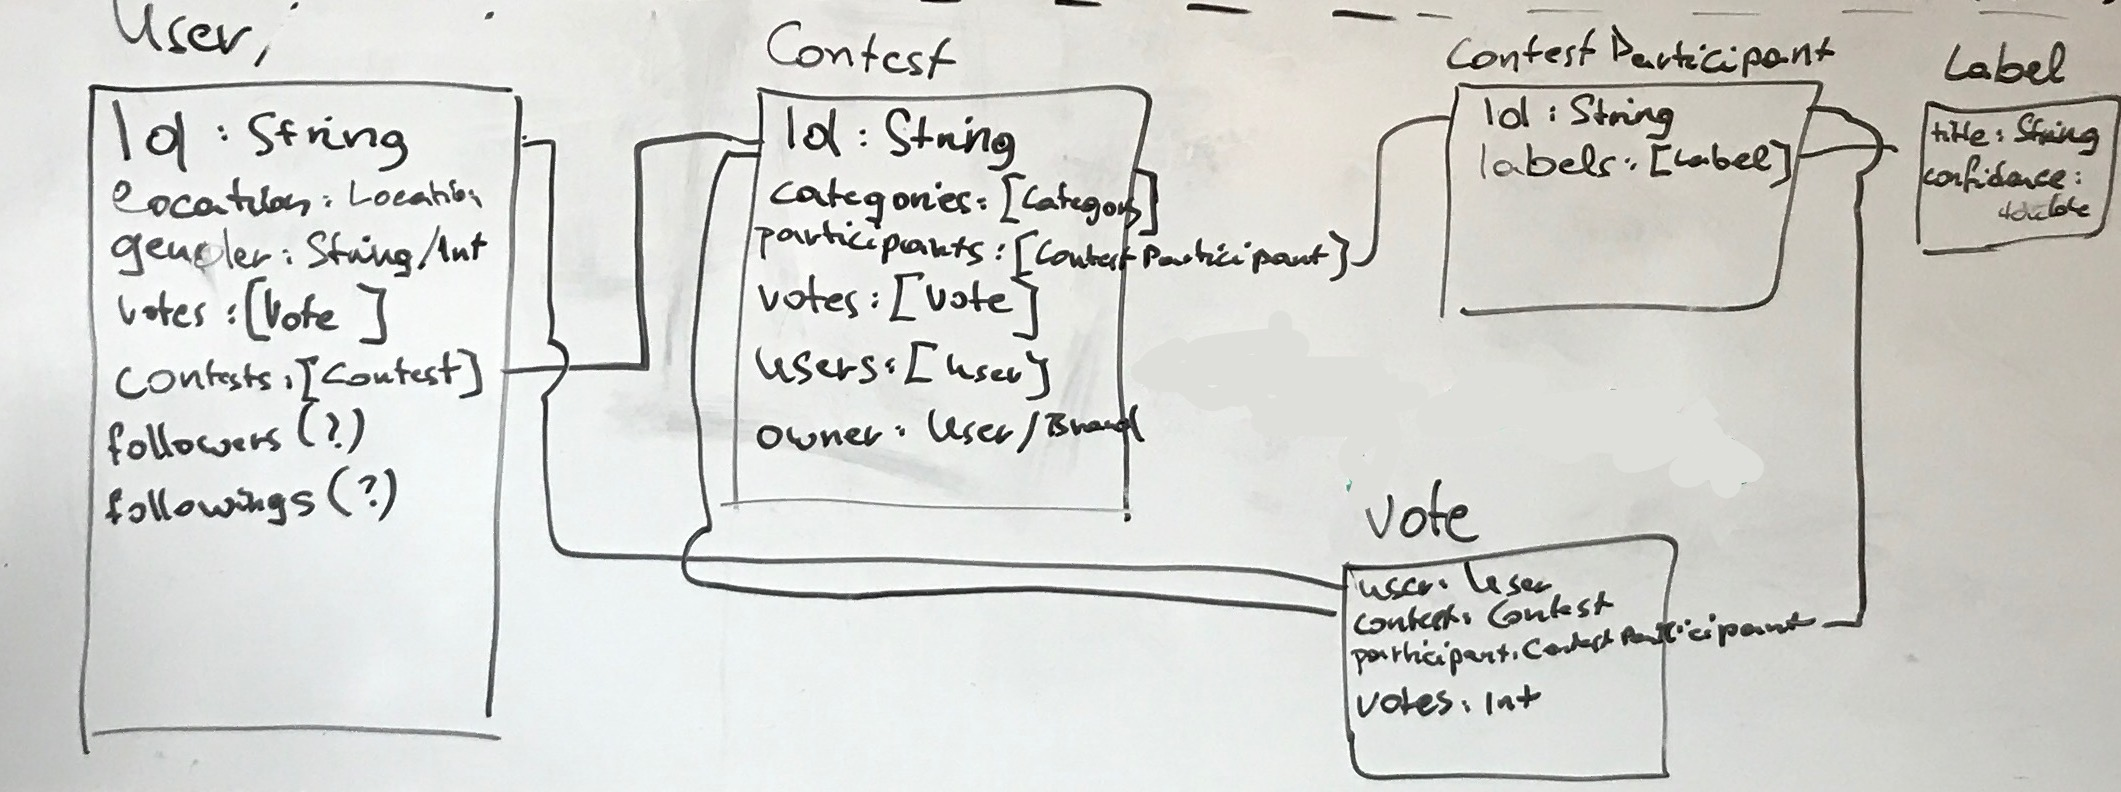
\includegraphics[width=0.8\textwidth]{Images/data_structure_whiteboard.jpg}
			\caption{The structure of the data models of the Choicely platform.}
			\label{choicely_data_models}
		\end{center}
    \end{figure}